\chapter{Introduction}
\label{cha:Intro}

\section{Field of Research}

Fractal geometry is an area of mathematical research that concerns itself with mathematically describing n-dimensional geometries - limited here to geometries on a plane - that display \textit{interesting} characteristics. 

Figure \ref{fig:flosnek} shows a rendering of one such geometry called \textsc{Gosper's flowsnake}.
It is a single, uninterrupted curve on a triangular grid, which displays the following characteristics

\begin{description}
	\item [Self-Similarity] The macroscopic behaviour of the curve is the same as its microscopic behaviour
	\item [Self-Avoidance] The curve is made from one continuous line, that never intersects with itself.
	\item [Area-Filling] The curve travels across every cell of its grid, i.e. it fills up a given, arbitrary area completely
\end{description}

\begin{figure}[h]
\centering
\begin{subfigure}{.33\textwidth}
  \centering
  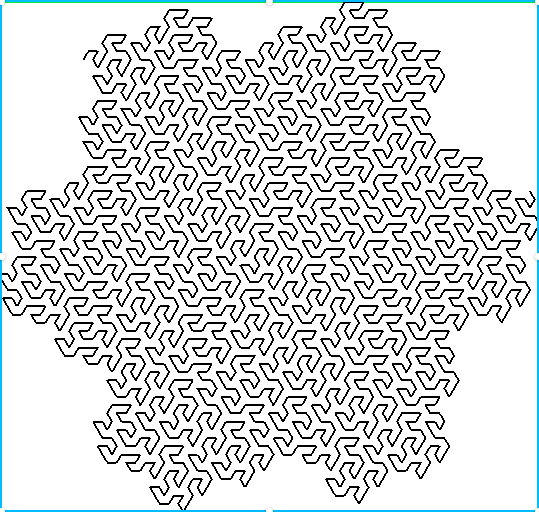
\includegraphics[width=.7\linewidth]{flosnek_4it}
  \caption{4 iterates}
\end{subfigure}%
\begin{subfigure}{.33\textwidth}
  \centering
  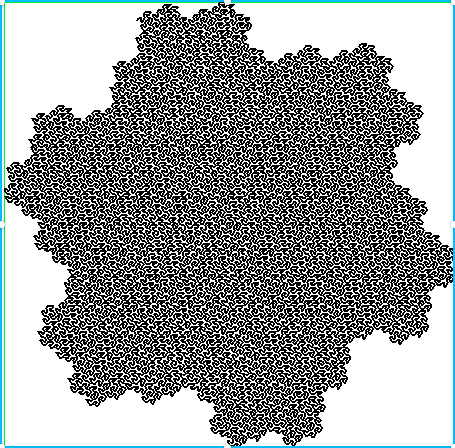
\includegraphics[width=.7\linewidth]{flosnek_5it}
  \caption{5 iterates, rescaled}
\end{subfigure}%
\begin{subfigure}{.33\textwidth}
  \centering
  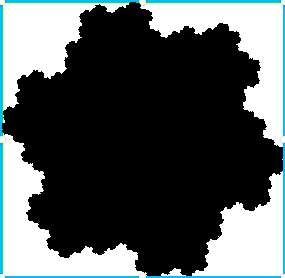
\includegraphics[width=.7\linewidth]{flosnek_8it}
  \caption{8 iterates, rescaled}
\end{subfigure}
\caption{Rendering of \textsc{Gosper's flowsnake}, with \gls{bounding box}}
	\label{fig:flosnek}
\end{figure}

The curve is generated by iterating a set of abstract substitution rules called \gls{lsys}.
The \gls{lsys} for figure \ref{fig:flosnek} is given in \citet{Arndt2016} to be 
\begin{quote}
	\centering
	L $\rightarrow$ L+R++R-L--LL-R+ \quad and \quad R $\rightarrow$ -L+RR++R+L--L-R
\end{quote}
starting with an initial string -  called \gls{axiom} - of L. The first iterate of \textsc{Gosper's flowsnake} thus becomes L+R++R-L--LL-R+, as the initial \gls{axiom} L gets substituted as per the rule. 
On each iteration the current string - called product - is substituted according to the given rules.

The characters in this string are given special meaning w.r.t. to the curve:
\begin{description}
	\item[Alphabetic character] Denotes drawing a line from the current position forward by on a defined length. Forward being defined as the current direction
	\item[+ -] Charactes denoting changes in direction by a set amount, e.g. in figure \ref{fig:flosnek} by $\pm60^\circ$, creating a triangular grid of movement
\end{description}

Those rules (among other, auxilliary ones discussed in \ref{sec:implementation}) define a way to render a curve given by an \gls{lsys} \gls{product}.

A curve is called a \gls{pfc}, if it will fill all of the 2D plane without self-intersecting, when the process of iterating its \gls{lsys} is repeated an infintely.

\section{Problem Statement}
In 2016, Prof. Jörg Arndt, the supervisor of this thesis, conducted research on finding \gls{pfc}s for \gls{lsys} with one non-constant character and published an article \citep{Arndt2016}, where he presented 2D renderings of the \gls{pfc}s found.

The tools used to get from an \gls{lsys} description to a graphical, pdf-embeddable rendering of the iterated curve were assortments of chained commandline scripts, leaving much to be desired in flexibility and ease-of-use.

Thus, a request was issued for the creation of a \emph{cross-platform, maintainable and extensible} software that is able to create, visualize and export \gls{pfc}s from their \gls{lsys} descriptions.

\section{Approach}

Since this problem is multi-faceted, and the additional requirements introduce significant complexity on top of the "implement a renderer/exporter" core task, a structured approach to finding a solution is taken using decomposition methods from software engineering.

First, the requirements are formulated and discussed.

Then, research is conducted on available technologies for satisfying given requirements.

An architectural model is created using \gls{uml} to define the system architecture.

This model ist then implemented and refined/amended to address issues arising during the implementation process.

The software is tested during development with \gls{ci} and \gls{Unit Testing} techniques.

Finally, a short investigation of application performance is conducted.

\section{Requirements to a Solution}
The following requirements to a satisfactory solution are given in figure \ref{fig:directreq} with a supposed workflow shown in the use-case diagram \ref{fig:uc}

\begin{figure}[h]
	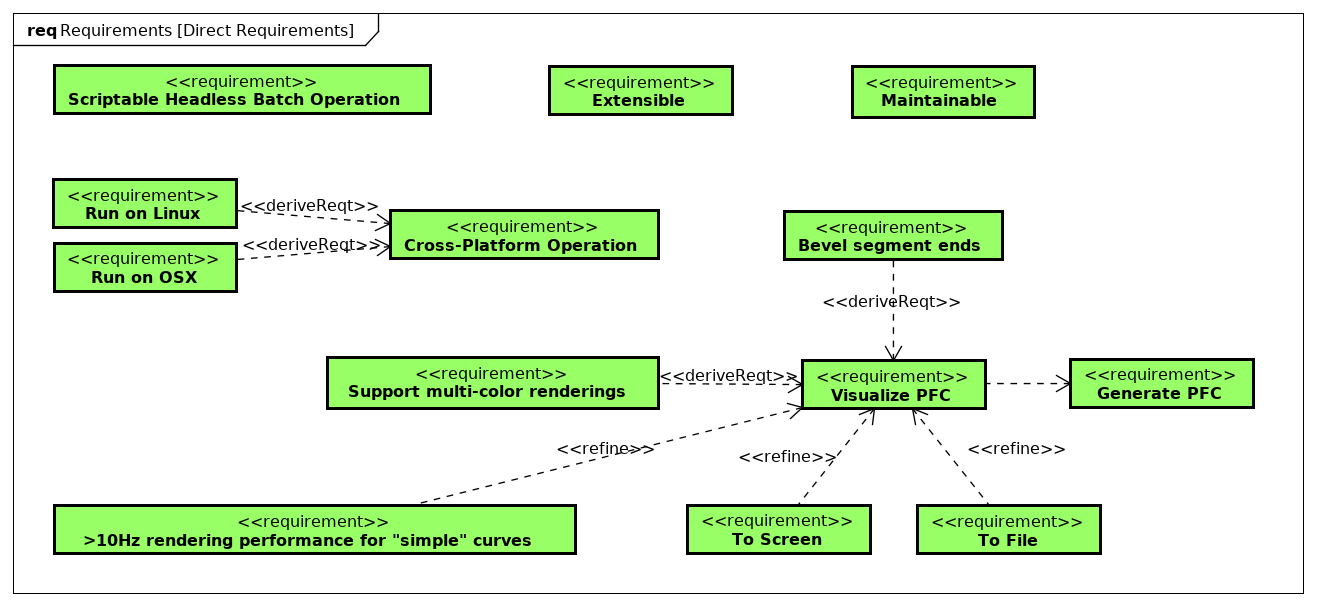
\includegraphics[width=\textwidth]{DirectRequirements}
	\caption{Direct user requirements to a solution}
	\label{fig:directreq}
\end{figure}


\begin{figure}
	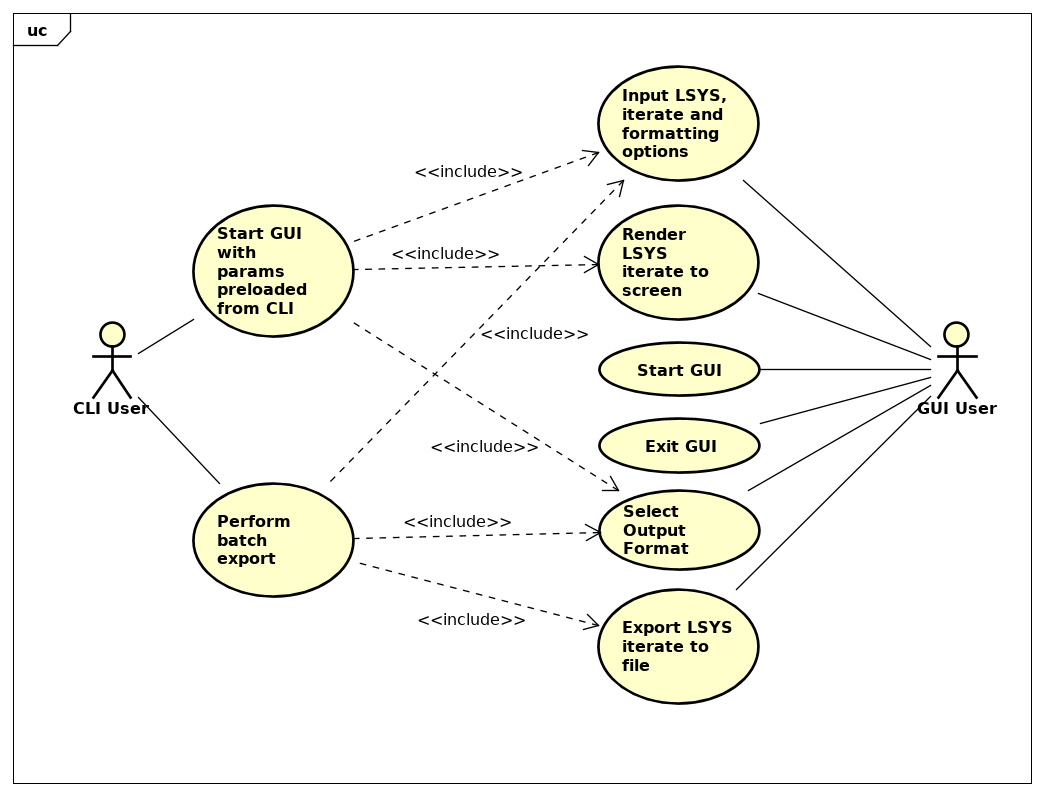
\includegraphics[width=\textwidth]{UseCaseDiagram}
	\caption{Workflow with the pfcrender tool}
	\label{fig:uc}
\end{figure}

These requirements are discussed in detail in the following sections and an architecture is formulated that satisfies them.
